%
% $XORP: xorp/docs/rib/rib.tex,v 1.31 2009/01/09 19:21:01 jtc Exp $
%

\documentclass[11pt]{article}

%\usepackage[dvips]{changebar}

\usepackage{subfigure}
\usepackage{fullpage}
\usepackage{setspace}
\usepackage{times}
\usepackage{latexsym}
\usepackage{epsfig}
\usepackage{graphicx}
\usepackage{xspace}
\usepackage{color}
\usepackage{amsmath}
\usepackage{rotating}
\usepackage{moreverb}
\usepackage{listings}
\usepackage{alltt}
\usepackage{stmaryrd}
%\usepackage[dvipdf]{graphics}
%\usepackage[dvips]{graphicx}
%\usepackage{xorp}

\definecolor{gray}{rgb}{0.5,0.5,0.5}
\newcommand{\etc}{\emph{etc.}\xspace}
\newcommand{\ie}{\emph{i.e.,}\xspace}
\newcommand{\eg}{\emph{e.g.,}\xspace}
%\newcommand{\comment}[1]{{\color{gray}[\textsf{#1}]}}
%\newcommand{\comment}[1]{}

% Changebar stuff
% \newenvironment{colorcode}{\color{blue}}{}
% \renewcommand{\cbstart}{\begin{colorcode}}
% \renewcommand{\cbend}{\end{colorcode}}

% \pagestyle{empty}

\begin{document}

\title{XORP Routing Information Base (RIB) Process \\
\vspace{1ex}
Version 1.8-CT}
\author{ XORP, Inc. and individual contributors		\\
         {\it http://www.xorp.org/}			\\
	 {\it xorp-users@xorp.org}
}
\date{June 1, 2010}

\maketitle


%%%%%%%%%%%%%%%%%%%%%%%%%%%%%%%%%%%%%%%%%%%%%%%%%%%%%%%%%%%%%%%%%%%%%%%
\section{Introduction}

This document provides an overview of the XORP Routing Information
Base (RIB) process.  It is intended to provide a starting point for
software developers wishing to understand or modify this software.

The RIB process takes routing information from multiple routing
protocols, stores these routes, and decides which routes should be
propagated on to the forwarding engine.  The RIB performs the following
tasks:

\begin{itemize}

  \item Stores routes provided by the routing protocols running on a XORP
  router.

  \item If more than one routing protocol provides a route for the same
  subnet, the RIB decides which route will be used.

  \item The winning unicast routes are propagated to the Forwarding
  Engine Abstraction (FEA) process and hence on to the forwarding
  engine. Multicast routes are not propagated to the FEA - they are only
  used to provide topology information to multicast routing protocols.

  \item Protocols such as BGP may supply to the RIB routes that have a
  nexthop that is not an immediate neighbor.  Such nexthops are resolved
  by the RIB so as to provide a route with an immediate neighbor to the
  FEA.

  \item Protocols such as BGP need to know routing metric and
  reachability information to nexthops that are not immediate neighbors.
  The RIB provides a way to register interest in such routing
  information, in such a way that the routing protocol will be notified
  if a change occurs.

  \item Protocols such as RIB need to announce routes to the neighbors
  (\eg routes from directly connected subnets, static routes, etc).
  The RIB provides the mechanism for redistributing the routes from
  a specific table to parties that have registered interest in that
  table.

\end{itemize}

By default, the RIB process holds four separate RIBs:

\begin{itemize}
  \item Unicast IPv4 RIB
  \item Unicast IPv6 RIB
  \item Multicast IPv4 RIB
  \item Multicast IPv6 RIB
\end{itemize}

C++ templates are used to build specialized IPv4 and IPv6 versions
from the same code.  Routing protocols such as Multiprotocol BGP are
capable of supplying routes that are multicast-only, and these would
be stored in the multicast RIBs.  The unicast and multicast RIBs
primarily differ in that only unicast routes are propagated to the
forwarding engine.

Note that we do not currently support multiple RIBs for other
purposes, such as VPN support, but the RIB architecture will permit
such extensions.

\section{Structure of a RIB}
The RIB process may hold multiple RIBs.  Figure~\ref{fig:rib_overview} gives
an overview of the structure of a unicast RIB.

\begin{figure}[htb]
  \centerline{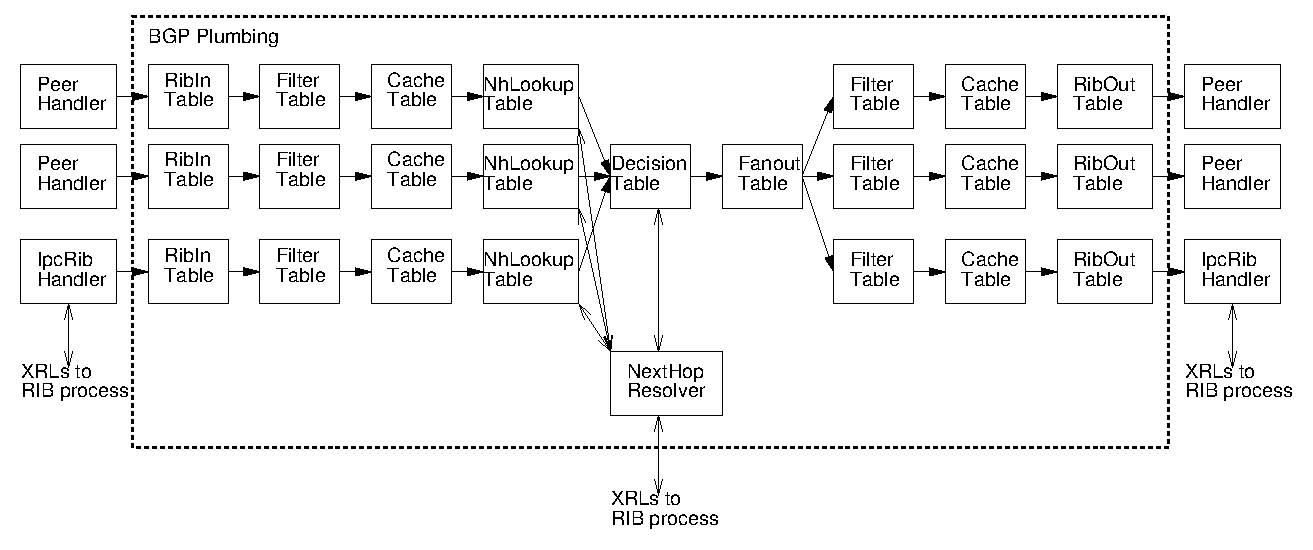
\includegraphics[width=1.0\textwidth]{figs/overview.ps}}
  \vspace{.05in}
  \caption{\label{fig:rib_overview}Overview of a RIB}
\end{figure}

In general, routing protocols supply routes to the OriginTables.
These routes then flow though the tree structure from left to right,
until they reach the RedistTable, where they are propagated to the
Forwarding Engine Abstraction (FEA) process.

%%%%%%%%%%%%%%%%%%%%%%%%%%%%%%%%%%%%%%%%%%%
\subsection{Plumbing}

The RIB plumbing code dynamically creates and maintains the tree of
tables as shown in Figure~\ref{fig:rib_overview}.  When a new routing protocol
registers with the RIB, a new OriginTable will be created, and a
MergeTable or an ExtIntTable will be created to plumb that OriginTable
into the RIB tree at an appropriate location.  Similarly, if a routing
protocol deregisters with the RIB, the relevant OriginTable and
additional tables will be deleted and the RIB tree simplified again.

%%%%%%%%%%%%%%%%%%%%%%%%%%%%%%%%%%%%%%%%%%%
\subsection{OriginTable}

The OriginTable accepts {\tt route\_add} requests from a single routing
protocol, stores the route, and propagates it downstream.  It also
answers {\tt lookup\_route} requests from downstream from the routes it
has stored.

An OriginTable for the ``connected'' protocol always exists, to handle
routes for directly connected interfaces.  It gets its information
via the VifManager from the Forwarding Engine Abstraction (FEA)
process.

%%%%%%%%%%%%%%%%%%%%%%%%%%%%%%%%%%%%%%%%%%%
\subsection{MergeTable}

A MergeTable has two upstream (parent) tables and one downstream
(child) table.

Multiple OriginTables may hold different routes for the same subnet.
Thus, when an {\tt add\_route} request reaches a MergeTable from one
parent, the MergeTable performs a route lookup on the other parent to
see if the route already exists.  If it does, then the new route is
only propagated if it is better than the existing route, where
``better'' is determined based on the relative administrative distance
of the routes.

Similarly, if a {\tt delete\_route} request reaches a MergeTable, it
performs a route lookup on the other parent table.  If the route being
deleted was better than the alternative, then the delete is propagated
downstream followed by an {\tt add\_route} for the alternative.  If the
route being deleted was worse than the alternative, then the deletion
needs to be propagated no further.

When a MergeTable receives a {\tt lookup\_route} request from
downstream, it sends the request on to both parents.  The better of
the two answers is sent in response.

%%%%%%%%%%%%%%%%%%%%%%%%%%%%%%%%%%%%%%%%%%%
\subsection{ExtIntTable}

ExtIntTable functions very similarly to the MergeTable, but there is
an asymmetry between the parents.  On the Internal side, the
originating routing protocols always supply routes that have an
immediate neighbor as the nexthop.  On the External side, the
originating routing protocols may supply routes that have an immediate
neighbor as the nexthop, but they may also supply routes where the
nexthop is multiple IP hops away.  

When an {\tt add\_route} request arrives from the external parent, the
ExtIntTable does the same comparisons that happen with a MergeTable.
However, it also checks to see if the nexthop is an immediate
neighbor.  If it is not, then the ExtIntTable attempts to find a route
that indicates which immediate neighbor to use to reach the nexthop,
and the nexthop in the route that is propagated downstream will be
that of this immediate neighbor.  If no route exists to the nexthop,
the route will not be propagated downstream, but will be stored in a
table of unresolved routes in case a route that arrives later can
cause it to resolve.

Each RIB only contains a single ExtIntTable.

%%%%%%%%%%%%%%%%%%%%%%%%%%%%%%%%%%%%%%%%%%%
\subsection{RegisterTable}

RegisterTable takes registrations from routing protocols for routing
information related to specific destinations, answers the request, and
stores the registration.  If the routing information in the
answer changes, it will asynchronously notify the routing protocol of
the change.  The precise interface is described in section \ref{reg},
but the general idea is illustrated by this example:

Suppose the RIB contains routes for 1.0.0.0/16 and 1.0.2.0/24.  Now a
routing protocol expresses an interest in address 1.0.1.1.  This
matches against the routing entry for 1.0.0.0/16, so the answer contains
1.0.0.0/16 and the related nexthop and metric.

However we would like the routing protocol to be able to use the
answer if it also cares about other addresses, such as 1.0.0.1 or
1.0.2.1.  However, while the former matches against 1.0.0.0/16, the
latter matches against 1.0.2.0/24.  Thus if the RIB only returns
1.0.0.0/16, the routing protocol cannot tell whether it can use this
information for any other address than the one it asked about.

To rectify this, the RIB returns not only the answer (1.0.0.0/16, plus
metric and nexthop), but also the subset of this prefix for which the
answer is known to be good.  In this case, the answer is good for
1.0.0.0 to 1.0.1.255, which is returned as a subnet: 1.0.0.0/23.
Any address that the routing protocol cares about that falls within
1.0.0.0/23 does not require additional communication with the RIB.

The RegisterTable keeps track of which information it gave which
routing protocol, so that if this information becomes invalid, the
routing protocol can be informed.  For example, if a new route appears
for 1.0.1.0/24, then this would cause the registration covering
1.0.0.0/23 to be invalidated because 1.0.1.0/24 is more specific than
1.0.0.0/16 and overlaps the range 1.0.0.0/23 of the registration.

Each RIB only contains a single RegisterTable.

%%%%%%%%%%%%%%%%%%%%%%%%%%%%%%%%%%%%%%%%%%%
\subsection{RedistTable}

The purpose of a RedistTable is to redistribute the routes from any RIB
table to all external parties that have registered interest at that
table. Thus, a RedistTable can be used for the redistribution of the
configured (and possibly filtered) routes from one routing protocol to
another.  For example, routes from within an AS might be propagated from
OSPF to BGP for external advertisement.

A RedistTable can by dynamically plumbed into the tree of tables at any
point, and there may be many RedistTables in each RIB. Typically,
RedistTables are inserted immediately after an OriginTable, and at the
end of the tree of tables.

ResistTables are used also for redistributing the final routes to the
FEA and other interested processes. Both the unicast and multicast RIBs
have a RedistTable at the end (see Figure~\ref{fig:rib_overview}).

%%%%%%%%%%%%%%%%%%%%%%%%%%%%%%%%%%%%%%%%%%%%%%%%%%%%%%%%%%%%%%%%%%%%%%%
\section{XRL Interface}

The RIB supports the following XRLs.

%%%%%%%%%%%%%%%%%%%%%%%%%%%%%%%%%%%%%%%%%%%
\subsection{Routing Protocol Registration}

\begin{verbatim}
add_igp_table4 ? protocol:txt & target_class:txt & target_instance:txt
               & unicast:bool & multicast:bool
add_igp_table6 ? protocol:txt & target_class:txt & target_instance:txt
               & unicast:bool & multicast:bool
add_egp_table4 ? protocol:txt & target_class:txt & target_instance:txt
               & unicast:bool & multicast:bool
add_egp_table6 ? protocol:txt & target_class:txt & target_instance:txt
               & unicast:bool & multicast:bool
delete_igp_table4 ? protocol:txt & target_class:txt & target_instance:txt
               & unicast:bool & multicast:bool
delete_igp_table6 ? protocol:txt & target_class:txt & target_instance:txt
               & unicast:bool & multicast:bool
delete_egp_table4 ? protocol:txt & target_class:txt & target_instance:txt
               & unicast:bool & multicast:bool
delete_egp_table6 ? protocol:txt & target_class:txt & target_instance:txt
               & unicast:bool & multicast:bool
\end{verbatim}

These XRLs are used by routing protocols to register with the RIB
process, and hence to create OriginTables in all the RIBs.

The {\tt \_igp\_} xrls will plumb the OriginTable on the Internal side
of the ExtIntTable.  The {\tt \_egp\_} xrls will plumb the OriginTable
on the External side of the ExtIntTable.

{\tt protocol} is a text string used to identify the routing protocol.
Currently it MUST be a protocol the RIB knows about, or an
administrative distance cannot be assigned to the routes.  Future
versions of the RIB may make this interface more extensible.

{\tt target\_class} and {\tt target\_instance} specify the
class and instance associated with the target.

{\tt unicast} and {\tt multicast} indicate whether the routing
protocol will insert routes into the unicast RIB or the multicast RIB
or both.

%%%%%%%%%%%%%%%%%%%%%%%%%%%%%%%%%%%%%%%%%%%
\subsection{Adding and Deleting Routes}

\begin{verbatim}
add_route4      ? protocol:txt & unicast:bool & multicast:bool  \
                & network:ipv4net & nexthop:ipv4 & metric:u32   \
                & policytags:list

add_route6      ? protocol:txt & unicast:bool & multicast:bool  \
                & network:ipv6net & nexthop:ipv6 & metric:u32   \
                & policytags:list

replace_route4  ? protocol:txt & unicast:bool & multicast:bool  \
                & network:ipv4net & nexthop:ipv4 & metric:u32   \
                & policytags:list

replace_route6  ? protocol:txt & unicast:bool & multicast:bool  \
                & network:ipv6net & nexthop:ipv6 & metric:u32   \
                & policytags:list

delete_route4   ? protocol:txt & unicast:bool & multicast:bool  \
                & network:ipv4net

delete_route6   ? protocol:txt & unicast:bool & multicast:bool  \
                & network:ipv6net

add_interface_route4    ? protocol:txt                          \
                        & unicast:bool & multicast:bool         \
                        & network:ipv4net & nexthop:ipv4        \
                        & ifname:txt & vifname:txt & metric:u32 \
                        & policytags:list

add_interface_route6    ? protocol:txt                          \
                        & unicast:bool & multicast:bool         \
                        & network:ipv6net & nexthop:ipv6        \
                        & ifname:txt & vifname:txt & metric:u32 \
                        & policytags:list

replace_interface_route4 ? protocol:txt                         \
                        & unicast:bool & multicast:bool         \
                        & network:ipv4net & nexthop:ipv4        \
                        & ifname:txt & vifname:txt & metric:u32 \
                        & policytags:list

replace_interface_route6 ? protocol:txt                         \
                        & unicast:bool & multicast:bool         \
                        & network:ipv6net & nexthop:ipv6        \
                        & ifname:txt & vifname:txt & metric:u32 \
                        & policytags:list
\end{verbatim}

These XRLs are used to communicate new routes, changed routes, or the
deletion of routes to the RIB.
The {\tt add\_interface\_route} and {\tt replace\_interface\_route}
XRLs are similar to the {\tt add\_route} and {\tt replace\_route}
XRLs except that the origin explicitly specifies the outgoing
network interface and vif for the route.

Note that sending an {\tt add\_route} for a route that is already in
the OriginTable for that protocol is an error, as is sending a {\tt
replace\_route} or {\tt delete\_route} for a route that is not in the
OriginTable for that protocol.

%%%%%%%%%%%%%%%%%%%%%%%%%%%%%%%%%%%%%%%%%%%
\subsection{Route Lookup}

\begin{verbatim}
lookup_route_by_dest4 ? addr:ipv4 & unicast:bool & multicast:bool 
        -> nexthop:ipv4
lookup_route_by_dest6 ? addr:ipv6 & unicast:bool & multicast:bool 
        -> nexthop:ipv6
\end{verbatim}

These XRLs may be used to see how the RIB would route a packet for a
specific destination.

{\tt nexthop} will return the resolved nexthop if the request is successful,
or all zeros otherwise.  It is an error for the unicast and multicast
fields to both be true or both false.

%%%%%%%%%%%%%%%%%%%%%%%%%%%%%%%%%%%%%%%%%%%
\subsection{VIF Management (test interface)}

\begin{verbatim}
new_vif ? name:txt
add_vif_addr4 ? name:txt & addr:ipv4 & subnet:ipv4net
add_vif_addr6 ? name:txt & addr:ipv6 & subnet:ipv6net
\end{verbatim}

These XRLs can be used to inform the RIB about directly connected
(virtual) interfaces.  The use of these XRLs is intended only for
testing purposes - the RIB normally learns of VIFs directly from the
FEA process.

%%%%%%%%%%%%%%%%%%%%%%%%%%%%%%%%%%%%%%%%%%%
\subsection{Route Redistribution}

\begin{verbatim}
redist_enable4 ? to_xrl_target:txt & from_protocol:txt & unicast:bool
               & multicast:bool & cookie:txt
redist_enable6 ? to_xrl_target:txt & from_protocol:txt & unicast:bool
               & multicast:bool & cookie:txt
redist_disable4 ? to_xrl_target:txt & from_protocol:txt & unicast:bool
               & multicast:bool & cookie:txt
redist_disable6 ? to_xrl_target:txt & from_protocol:txt & unicast:bool
               & multicast:bool & cookie:txt
redist_transaction_enable4 ? to_xrl_target:txt & from_protocol:txt
               & unicast:bool & multicast:bool & cookie:txt
redist_transaction_enable6 ? to_xrl_target:txt & from_protocol:txt
               & unicast:bool & multicast:bool & cookie:txt
redist_transaction_disable4 ? to_xrl_target:txt & from_protocol:txt
               & unicast:bool & multicast:bool & cookie:txt
redist_transaction_disable6 ? to_xrl_target:txt & from_protocol:txt
               & unicast:bool & multicast:bool & cookie:txt
\end{verbatim}

These XRLs are intended to be used to enable and disable route
redistribution from a RIB table to an XRL target.
The {\tt *\_transaction\_*} XRLs are used for registering interest in
transaction-based route redistribution (\ie where there is
{\tt start\_transaction} and {\tt commit\_transaction} around each block
of add/delete routes).

%%%%%%%%%%%%%%%%%%%%%%%%%%%%%%%%%%%%%%%%%%%
\subsection{Registration of Interest in Routes}
\label{reg}

\begin{verbatim}
register_interest4 ? target:txt & addr:ipv4 
        -> resolves:bool & base_addr:ipv4 & prefix_len:u32 & 
           real_prefix_len:u32 & nexthop:ipv4 & metric:u32
register_interest6 ? target:txt & addr:ipv6 
        -> resolves:bool & base_addr:ipv6 & prefix_len:u32 & 
           real_prefix_len:u32 & nexthop:ipv6 & metric:u32
deregister_interest4 ?  target:txt & addr:ipv4 & prefix_len:u32
deregister_interest6 ?  target:txt & addr:ipv6 & prefix_len:u32
\end{verbatim}

These XRLs are used to register and deregister interest in routing
information related to a specific IP address. 

Target is the name of the XRL module that registered the interest.

{\tt resolves} indicates whether or not the address is routable.  If
it is not routable, the values of {\tt nexthop} and {\tt metric} are
undefined.  {\tt real\_prefix\_len} returns the prefix length of the routing
entry that matches the address in the request.  {\tt prefix\_len} returns
the prefix length of the largest subnet that covers the address and is
not overlayed by a more specific route.  Thus ${\tt prefix\_len} >= {\tt
real\_prefix\_len}$ and {\tt addr} is an address within the subnet {\tt
base\_addr/prefix\_len} which itself is a subset of the subnet {\tt
base\_addr/real\_prefix\_len}.  

The routing protocol need not ask again for any address that lies
within {\tt base\_addr/prefix\_len} but can not use this answer to determine
anything about addresses that lie outside of {\tt base\_addr/prefix\_len}
but within {\tt base\_addr/real\_prefix\_len}.

\subsection{Registration of Interest in Routes: Client Interface}
When a routing protocol has registered interest in routes, the RIB
will need to be able to asynchronously call the routing protocol to
inform it of any changes.  Thus the routing protocol must implement
the rib client interface.  This consists of the following XRLs:
\begin{verbatim}
route_info_changed4 ? addr:ipv4 & prefix_len:u32 & 
        nexthop:ipv4 & metric:u32
route_info_changed6 ? addr:ipv6 & prefix_len:u32 & 
        nexthop:ipv6 & metric:u32

route_info_invalid4 ? addr:ipv4 & prefix_len:u32
route_info_invalid6 ? addr:ipv6 & prefix_len:u32
\end{verbatim}
The {\tt route\_info\_changed} XRLs inform the routing protocol that the
nexthop or metric associated with the route with subnet {\tt
addr/prefix\_len} has changed.  The registration with the RIB is still
valid.

The {\tt route\_info\_invalid} XRLs inform the routing protocol that the
information associated with the specified subnet is no longer correct.
The registration with the RIB is no longer valid, and the routing
protocol must re-register with the RIB to find out what happened.

%%%%%%%%%%%%%%%%%%%%%%%%%%%%%%%%%%%%%%%%%%%%%%%%%%%%%%%%%%%%%%%%%%%%%%%
%     APPENDIX
%%%%%%%%%%%%%%%%%%%%%%%%%%%%%%%%%%%%%%%%%%%%%%%%%%%%%%%%%%%%%%%%%%%%%%%
\appendix
\section{Modification History}

\begin{itemize}

  \item December 11, 2002: Initial version 0.1 completed.

  \item March 10, 2003: Updated to match XORP release 0.2:
   Added information about the ``connected'' OriginTable.

  \item June 9, 2003: Updated to match XORP release 0.3:
   Described the new RibClient registration mechanism.

  \item August 28, 2003: Updated to match XORP release 0.4:
   No changes.

  \item November 6, 2003: Updated to match XORP release 0.5:
   No changes.

  \item July 8, 2004: Updated to match XORP release 1.0:
   Replaced ExportTable with RedistTable. Fixed the XRLs specification.

  \item April 13, 2005: Updated to match XORP release 1.1.
   Fixed the XRL names. Added description for the add\_interface\_route and
   replace\_interface\_route XRLs.

  \item March 8, 2006: Updated to match XORP release 1.2:
   No significant changes.

  \item August 2, 2006: Updated to match XORP release 1.3:
   Added ``Modification History'' appendix.

  \item March 20, 2007: Updated to match XORP release 1.4:
   No changes.

  \item July 22, 2008: Updated to match XORP release 1.5:
   No changes.

\end{itemize}

%%%%%%%%%%%%%%%%%%%%%%%%%%%%%%%%%%%%%%%%%%%%%%%%%%%%%%%%%%%%%%%%%%%%%%%
%     BIBLIOGRAPHY
%%%%%%%%%%%%%%%%%%%%%%%%%%%%%%%%%%%%%%%%%%%%%%%%%%%%%%%%%%%%%%%%%%%%%%%
%\bibliography{xorp}
%\bibliographystyle{plain}

%%%%%%%%%%%%%%%%%%%%%%%%%%%%%%%%%%%%%%%%%%%%%%%%%%%%%%%%%%%%%%%%%%%%%%%
\end{document}
